\section{Longitudinal flow fluctuations}

\begin{itemize}
	\item longitudinal flow dynamics studied for first time at LHC
	\item CMS measurements of EP decorrelation~\cite{CMS-HIN-15-008}
	\item ATLAS measurements of magnitude and EP fluctuations~\cite{HION-2016-04}
	\item Currently decorrelation measurements show mostly linear decorrelation with eta, 
		    except in most central events.
	\item Major improvement due to increase of tracking acceptance in run-4 to +-4 units 
		    in eta will allow study of non-linear decorrelation.
	\item possibility of studying longitudinal flow fluctuations via PCA technique~\cite{Bhalerao:2014mua} done by CMS
\end{itemize}


\begin{figure*}[!htb]
\begin{center}
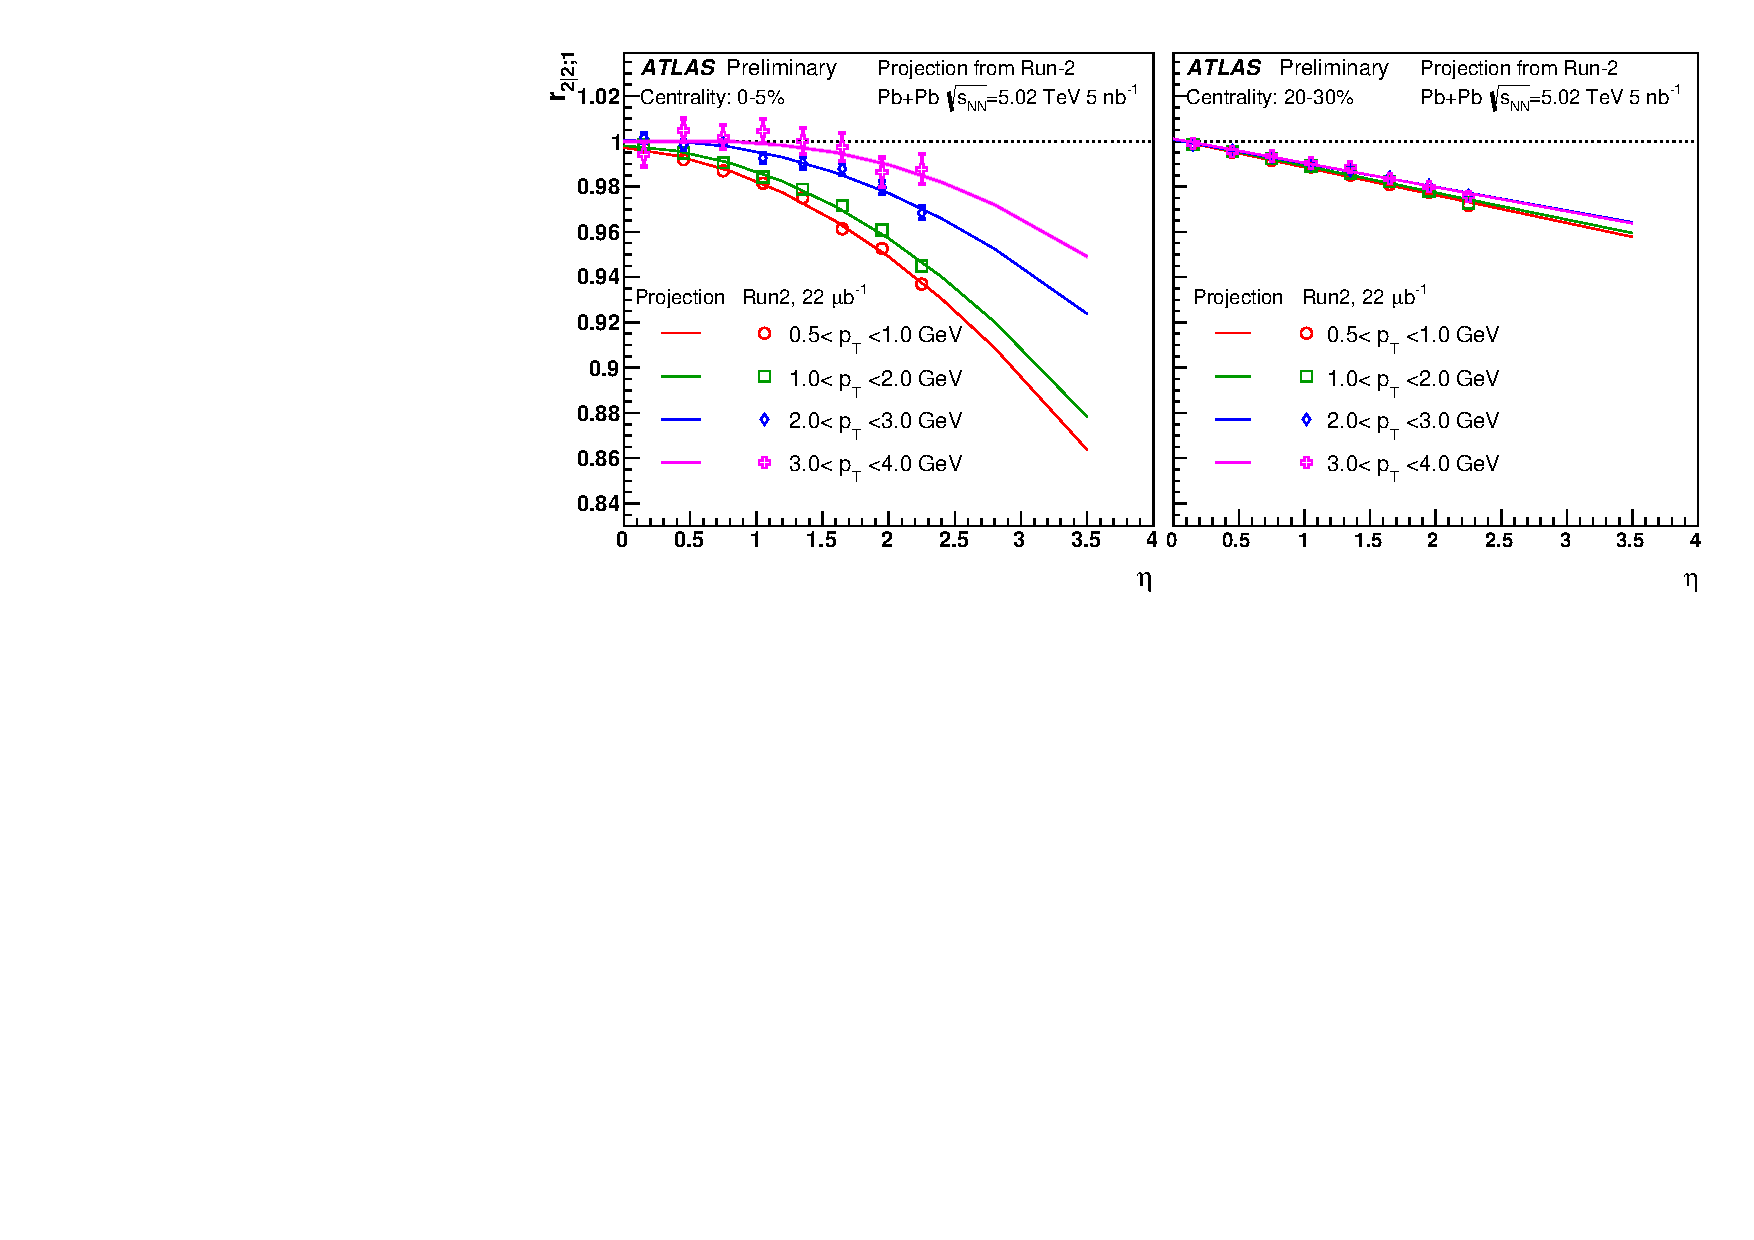
\includegraphics[width=0.8\textwidth]{figs/atlas_projection_r221}
\caption{
ATLAS projection plot of longitudinal flow decorrelation in Run-4 
	due to increased tracking acceptance.
}
\label{fig:atlas_r221}
\end{center}
\end{figure*}

